\chapter{Reconhecimento de voz}
\label{cap:speech-recognition}

Neste capítulo, abordaremos a parte teórica do reconhecimento de voz, sem nos preocuparmos com a forma de implementação ou sua aplicação no contexto deste trabalho. Em particular, analisaremos brevemente os principais parâmetros que influenciam seu uso.

% ---------------------------------------------------------------------

\section{Definição}

% https://en.wikipedia.org/wiki/Speech_recognition
% https://en.wikipedia.org/wiki/Computational_linguistics

\textbf{Reconhecimento automático de voz} (ou da fala), muitas vezes referido como \textit{speech to text} (\textbf{STT}), é um campo multidisciplinar que envolve as áreas de Inteligência Artificial, Estatística e Linguística. Busca-se desenvolver metodologias e tecnologias para que computadores sejam capazes de captar, reconhecer e traduzir a linguagem falada para texto.

% ---------------------------------------------------------------------

\section{História}

% https://nexbridge.co.uk/speech-recognition-in-the-21st-century/
% https://www.callcentrehelper.com/the-top-five-uses-of-speech-recognition-technology-1536.htm
% http://www.pcworld.com/article/243060/speech_recognition_through_the_decades_how_we_ended_up_with_siri.html
O primeiro sistema de reconhecimento de voz conhecido foi o \textit{Audrey}, construído em 1952 por três pesquisadores do \textit{Bell Labs} para reconhecer dígitos falados por um único usuário.

10 anos depois, a IBM apresentou o \textit{Shoebox}, que reconhecia 16 palavras em inglês, entre elas os dígitos de 0 a 9. Quando captava palavras como \textit{plus}, \textit{minus} ou \textit{total}, \textit{Shoebox} instruía outra máquina de adições a realizar cálculos ou imprimir o resultado. A entrada era feita por um microfone (figura \ref{shoebox}), que convertia a voz do usuário em impulsos elétricos, classificados internamente por um circuito de medição.


% Shoebox text: https://www-03.ibm.com/ibm/history/exhibits/specialprod1/specialprod1_7.html
% Image: http://www.cassiopeia.it/resources-2/computing-history-timeline/
\begin{figure}[H]
  \centering
  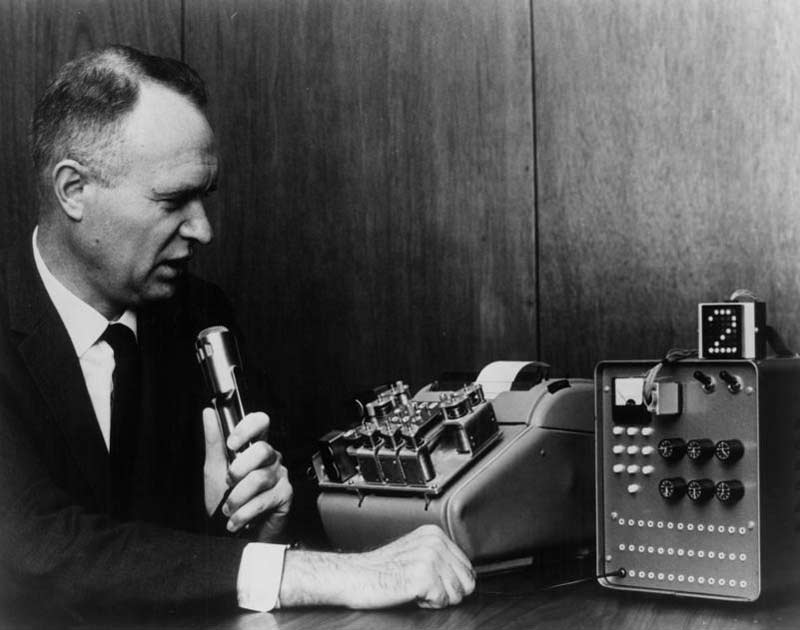
\includegraphics[width=.5\textwidth]{image/shoebox.jpg}
  \caption{Máquina \textit{Shoebox} sendo operada}
  \label{shoebox}
\end{figure}

Sistemas de reconhecimento de voz só tiveram um avanço realmente significativo na década de 80, devido a um método estatístico denominado \emph{modelo oculto de Markov} (ou \textbf{HMM}, sigla para \textit{Hidden Markov Model}). Ao invés de procurar por modelos de palavras em padrões de som, considera-se a probabilidade de um som desconhecido possuir palavras, o que acelerou o processo e tornou possível usar um vocabulário maior nos computadores. Veremos HMM com um pouco mais de detalhe na seção \ref{cap:hmm}.

Outro modelo que ganhou bastante popularidade na mesma época foi o de redes neurais, que é efetivo para classificar palavras isoladas e fonemas individuais mas encontra problemas em tarefas envolvendo reconhecimento contínuo. Ao contrário do HMM, este método não consegue modelar bem dependências temporais.

A evolução na tecnologia de reconhecimento de voz foi tamanha que, atualmente, é inegável seu impacto em nosso dia a dia. Um celular moderno consegue captar palavras ou pequenas frases de seu usuário dentre um enorme vocabulário para fazer buscas na Internet, tocar uma música ou fazer uma ligação. Muitas empresas utilizam máquinas para receber ligações de seus clientes; de acordo com o que interpretam, a chamada é redirecionada para um funcionário mais adequado. Alguns países chegam até a usar reconhecimento de voz para autenticar a identidade de alguém por telefone, com o objetivo de evitar fornecer dados pessoais pelo mesmo. Também há usos em transportes, na área médica e para fins educativos.

% ---------------------------------------------------------------------

\section{Componentes de um sistema genérico}

A figura \ref{generic-stt} apresenta os três componentes de um sistema genérico envolvendo STT:

\begin{itemize}
\item O \textbf{usuário} do sistema, que codifica um comando através de sua voz;

\item O \textbf{dispositivo} de STT, que converte a mensagem falada para um formato interpretável;

\item O \textbf{software de aplicação}, que recebe a saída do dispositivo e realiza uma ação apropriada.
\end{itemize}

% https://www.nap.edu/read/19357/chapter/4#10
\begin{figure}[H]
  \centering
  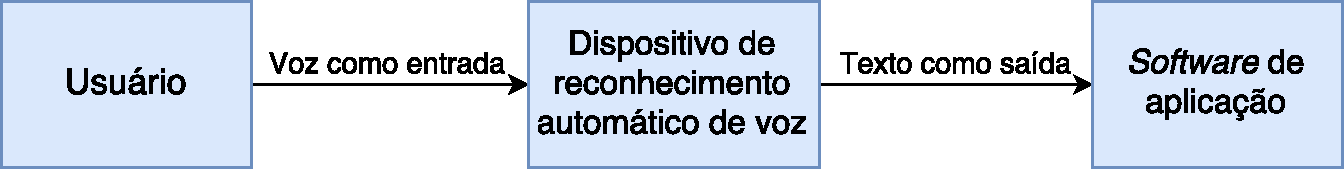
\includegraphics[width=.9\textwidth]{image/generic-stt.pdf}
  \caption{Sistema genérico de reconhecimento automático de voz}
  \label{generic-stt}
\end{figure}

% ---------------------------------------------------------------------

\section{Principais parâmetros}

% https://www.nap.edu/read/19357/chapter/4#10
% http://www.voice-commands.com/103.htm
Há diversos tipos de parâmetros que caracterizam as capacidades de um sistema de reconhecimento de voz, influenciando sua forma de funcionamento, eficiência e acurácia. A influência destes fatores varia de acordo com o tipo de aplicação que se deseja construir.

Os principais parâmetros são apresentados a seguir.

% ---------------------------------------------------------------------

\subsection{Fluência}

A fluência está relacionada à forma de se comunicar com o sistema. Tipicamente, a fala do usuário pode ser feita através de \emph{palavras isoladas}, com pausas entre elas; \emph{palavras conectadas}, que são concatenadas sem pausas; ou \emph{fala contínua}, onde o fluxo de palavras é semelhante a uma fala natural.

% ---------------------------------------------------------------------

\subsection{Dependência do usuário}

A dependência ou não do usuário classifica os sistemas em dois grupos:

% https://speechangel.com/2016/05/04/difference-speaker-dependent-speaker-independent-recognition-software
\begin{itemize}
\item Os sistemas \textbf{dependentes} (\textit{speaker-dependent}), caracterizados pelo \emph{treinamento} feito pelo usuário. Isto é, são computadores que analisam e se adaptam aos padrões particulares da fala captada, resultando em uma maior acurácia. Geralmente, o usuário deve ler algumas páginas de texto para a máquina antes de começar a usar o sistema. Esta variante é comumente usada em casos particulares, onde um número limitado de palavras deve ser reconhecido com bastante precisão.

\item Os sistemas \textbf{independentes} (\textit{speaker-independent}), que são desenvolvidos para reconhecer a voz de qualquer pessoa e não requerem treinamento. É a melhor opção para aplicações interativas que usam voz, já que não é viável fazer com que os usuários leiam páginas de texto antes do uso, ou para sistemas usados por diferentes pessoas. Sua desvantagem é a acurácia menor se comparado ao reconhecimento dependente; para contornar isso, costuma-se limitar o vocabulário reconhecido pelo sistema.
\end{itemize}

% ---------------------------------------------------------------------

\subsection{Vocabulário}

O vocabulário representa as palavras reconhecidas pelo sistema. Seu tamanho pode ser pequeno (menor que 20 palavras) até muito grande (mais de 20 mil palavras), sendo diretamente proporcional à velocidade do reconhecimento. Além disso, a similaridade entre a pronúncia de algumas palavras pode afetar a acurácia, uma vez que a distinção entre elas torna-se mais complicada.

% ---------------------------------------------------------------------

\subsection{Ambientais}

Parâmetros ambientais referem-se a fatores externos ao sistema que podem interferir no reconhecimento de voz. Destacam-se:

\begin{itemize}
\item A \textbf{relação sinal/ruído}, que avalia a intensidade média do sinal recebido em relação ao ruído de fundo, tipicamente medido em decibéis (dB). Quanto menor a taxa, maior a dificuldade no reconhecimento de voz.

\item O \textbf{próprio usuário}, o que inclui o volume de sua voz, a velocidade com que fala e até mesmo sua condição psicológica: o nível de estresse de um piloto sob ataque em uma aeronave é diferente de alguém simplesmente querendo ouvir uma música, por exemplo.
\end{itemize}
